\chapter{Simulations}

Les simulations numériques permettent de calculer les propriétés des systèmes là où la diagonalisation directe des hamiltoniens est trop difficile. Elle permet également de faire varier facilement les géométries et les potentiels dans les systèmes. Les algorithmes mis en jeu sont en général lents et peu efficients car ils essaient d'explorer l'ensemble de l'espace des configurations du système. Les modèles 1D que nous étudions dans cette thèse ont l'avantage d'être rapides à calculer et donnent une pléthore d'informations qui peuvent être extrapolées aux modèles 2D et 3D à basse température. 

\section{Algorithme de Metropolis}

Les systèmes à l'équilibre sont, en présence d'une température non-nulle, définis par les moyennes statistiques des grandeurs observables. La moyenne statistique de l'observable $A$ est définie vis-à-vis de la fonction de partition 
\begin{align}
	<A> = \sum_\mu e^{-\beta \mH(\mu)} = \sum_E e^{-\beta(E-T S)}
\end{align}
où $\sum_\mu$ désigne la somme sur tous les micro-états $\mu$ possibles du système et $\sum_E$ la somme sur toutes les énergies possibles du système associées à leur entropie $S$. Tandis qu'une diagonalisation de la fonction de partition nécessiterait de connaître tous les micro-états possibles, on observe que certains états sont plus probables que d'autres car d'énergie moindre, et donc contribuent plus aux moyennes statistiques que les autres états, tandis qu'à haute température la densité d'états de plus haute énergie contribue de manière plus importante à l'entropie.
Les algorithmes de Metropolis ont pour objectif d'explorer l'espace des phases de manière aléatoire afin de découvrir quelles configurations contribuent le plus aux observables du système, afin de converger vers la valeur limite $<A>(t=\infty) = <A>$.

Nous nous basons ici sur \cite{newman_monte_1999} afin d'expliquer le fonctionnement d'un tel algorithme.

Soit $\mu$ un micro-état de notre système d'énergie $E(\mu)$. À l'équilibre, la probabilité d'occupation du système est
\begin{align}
	p_\mu = \frac{1}{\mZ} e^{-\beta E(\mu)}
\end{align}
qui définit la fonction de partition $\mZ$. Dans un algorithme de Metropolis, on met à jour le micro-état en prenant un site $i$ au hasard
\footnote{L'utilisation d'un générateur de nombre aléatoire (\textit{pRNG}) efficace est primordial. Il est déconseillé d'utiliser le générateur standard \textit{default\_random\_engine} de la librairie C++ \textit{rand} et conseillé d'opter pour des générateurs \textit{sfc64} ou \textit{xoroshiro}. Pour un pRNG booléen performant, voir \url{https://martin.ankerl.com/2018/12/08/fast-random-bool/}. Pour accélérer encore plus les calculs, ne pas oublier d'utiliser le flag d'optimisation \textit{-O3}  sur \textit{gcc} si vous codez en C/C++. Tout cela combiné accélère le code d'un facteur 20 environ. \newline
De plus, bien que la librairire OpenMP pour paralléliser le code soit simple d'utilisation, elle gère très mal - de sa nature de mémoire partagée - les pRNG. Je conseille vivement l'utilisation de la librairie MPI qui assure une étanchéité au niveau des pRNG entre chaque thread.} 
et en le changeant légèrement vers un état $\nu$. Dans un système d'Ising, nous choisissons un spin $\sigma_i$ au hasard et regardons s'il peut être renversé ou échangé avec l'un de ses plus proches voisins. Dans le modèle SOS, nous choisissons une colonne $h_i$ au hasard et regardons s'il est possible d'ajouter ou de retirer une unité à la hauteur (c'est le nombre de particules sous l'interface au site $h_i$), ou d'échanger une particule d'une colonne vers une de ses plus proches voisins.
La différence d'énergie notée $\Delta E(\mu \rightarrow \nu)$ donne la probabilité de transition entre les deux. Si l'état final $\nu$ a une énergie inférieure à l'état initial, alors il est forcément plus probable que $\mu$, et nous acceptons le changement. Dans le cas où $E_\nu \greater E_\nu$, on accepte le changement avec une probabilité satisfaisant au bilan détaillé pour une marche markovienne satisfaint à l'état d'équilibre de Botlzmann
\begin{align}
\frac{p(\mu \rightarrow \nu)}{p(\nu \rightarrow \mu)} = e^{-\Delta Ep(\nu \rightarrow \mu)}
\end{align}
ce qui nous donne la probabilité de transition $\mu \to \nu$ de Metropolis
\begin{align}
	p(\mu \rightarrow \nu) = min(1,e^{-\beta \Delta E(\mu \rightarrow \nu)})
\end{align}
Ensuite on prend un nombre aléatoire $q$ entre $0$ et $1$. Si $q < p(\mu \rightarrow \nu)$, alors la transition est validée. Une étape de Monte Carlo est achevée lorsque $L$ tentatives de transition ont été faites. Cependant, il est possible d'accélérer l'algorithme en utilisant un temps continu \cite{newman_monte_1999} ou en prenant en compte les états dont la transition a été refusée \cite{frenkel_speed-up_2004}.
L'erreur obtenue à la fin sur notre observable $<A>$ au cours d'une simulation ayant duré $t_{max}$ étapes de Monte Carlo est 
\begin{align}
	E(A) = \sqrt{\frac{2 \tau}{t_{max}} (<A^2>-<A>^2)} 
\end{align}
Cette variance dépend du temps de corrélation $\tau$ puisque si deux micro-états sont très rapprochés dans le temps , l'observable en question n'aura pas grandement évolué. En pratique, il suffit que $\frac{\tau}{t_{max}} \less 10^{-4}$ pour obtenir une erreur inférieure à $1\%$. Ce temps de corrélation $\tau$ se calcule via la fonction d'auto-corrélation 
\begin{align}
\mC(t) = <A(t')A(t+t')>-\langle A \rangle^2 = \frac{1}{T_{max}}\int_0^{T_{max}}A(t')A(t+t')-<A>^2 dt' \simeq e^{-\frac{t}{\tau}}
\end{align}
qui se comporte comme une somme d'exponentielles, mais où dans la limite thermodynamique, seul le mode de relaxation le plus long compte\cite{wansleben_monte_1991}. En supposant la limite thermodynamique, l'ordre de grandeur de $\tau$ - et donc de la variance de nos observables - est donnée par le calcul de l'intégrale\footnote{Je recommande d'intégration de Simpson.}
\begin{align}
	\tau = \int_0^{\infty} \mC(t)/\mC(0) dt
	\label{tau_cor}
\end{align}
Le calcul de la plus grande longueur de corrélation $\xi$ du système se fait de manière analogue en intégrant la fonction de corrélation spatiale définie par
\begin{align}
\mC(x) = \frac{1}{L} \sum_{x'}^L A(x')A(x+x')-<A>^2 \simeq e^{-\frac{x}{\xi}}
\end{align}
Une discussion plus rigoureuse sur la forme de la fonction de corrélation spatiale sera donnée dans la section \ref{sec_laser}.

	\subsection{Ensemble grand-canonique : algorithme de Glauber}

\begin{figure}[h]
	\centering
	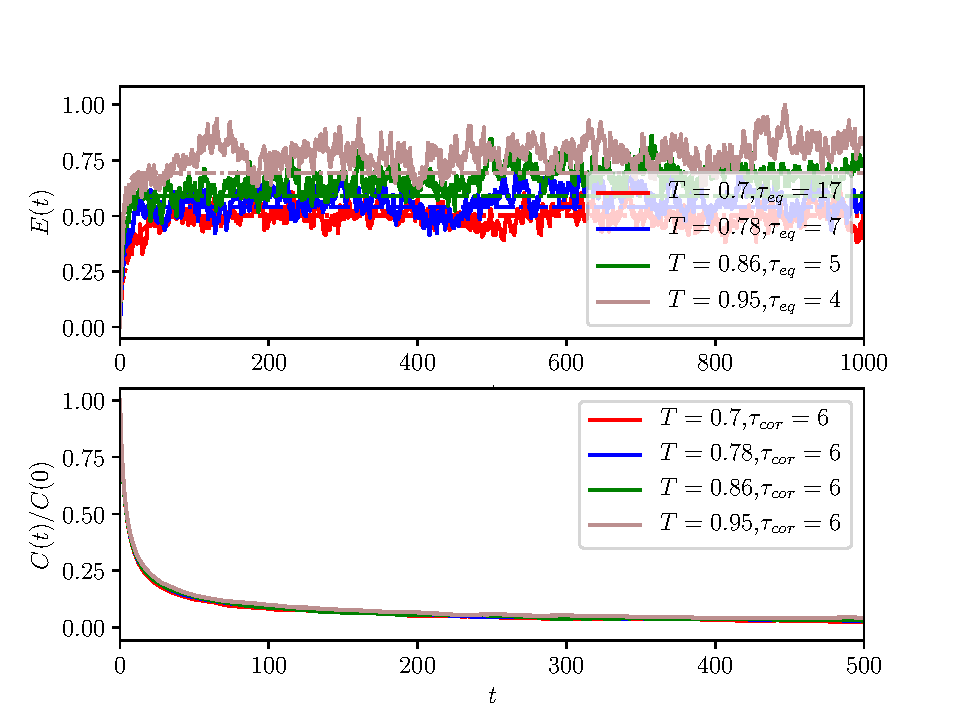
\includegraphics[scale=1]{numerical/sos-glau-eq-cor.pdf}
	\caption{Courbe de l'énergie (haut) et fonction d'auto-corrélation (bas) dans avec un \textbf{paramètre d'ordre non-conservé} à partir de la condition initiale. Le temps d'équilibrage (en étapes de Monte Carlo) diminue avec la température, tandis que le temps de corrélation reste relativement constant. Le temps de corrélation étant extrêmement faible, $10^7$ étapes de Monte Carlo suffisent à avoir une erreur de moins de $0.1\%$ sur les moyennes mesurées.}
	\label{eq-glau}
\end{figure}
	
Le dépôt de particules provenant d'un réservoir permet de faire grandir un cristal à partir d'un substrat. Ce genre de systèmes est défini par le potentiel chimique $\mu$ des particules, dans le solvant et appartient à l'ensemble grand-canonique. Dans ce cas, on choisit au hasard de manière uniforme une colonne $h_i$ dans laquelle on décide de mettre ou d'enlever une particule selon le flux de particules $\nu$ vu dans l'équation d'Edwards-Wilkinson \ref{edwards-wilkinson}. Si l'on se place à l'équilibre thermodynamique, c'est-à-dire qu'autant de particules se déposent au niveau de l'interface que de particules la quittent, alors il faut que la probabilité de ces deux événements soient égales entre elles, et donc égales à $50\%$.
Dans le cas où la géométrie est infinie, les valeurs des $h_i$ ne sont pas bornées, tandis que dans une géométrie torique de hauteur $L$, on rejette toutes les configurations qui ne respectent pas aux conditions $0 \leq h_i \leq L$.
En essayant d'aller du micro-état $\mu$ vers le micro-état $\nu$ où on a fait la transformation $h_i \rightarrow h_i + \alpha$ où $\alpha=\pm 1$, on obtient que la différence d'énergie est
\begin{align}
	\Delta E &= |h_{i-1}-(h_i \pm 1)| + |h_{i+1}-(h_i \pm 1)| - |h_{i-1}-h_i| - |h_{i+1}-h_i|  \\
		&= 2 \left( (h_i \leq h_{i-1}) + (h_i \geq h_{i+1}) -1 \right )
\end{align}
où $(h_i \leq h_{i-1})$ est un booléen valant $1$ si la condition est vraie, $0$ sinon.
Le changement de magnétisation est alors $\Delta M = \alpha$, et la largeur de l'interface, définie par $\sigma = \sum_i (h_i-h_{i+1})^2$, change comme
\begin{align}
	\Delta \sigma = 2 \alpha (h_{i+1}-h_i) + 2
\end{align}
On n'a donc pas besoin, à chaque pas de temps, de recalculer ces deux grandeurs, il suffit de les actualiser dans une variable pour avoir les observables à tout instant $t$.


Afin d'accélérer le processus d'équilibrage du système, il est recommandé de commencer directement avec la valeur moyenne de magnétisation calculée à partir de la matrice de transfert. On regarde ensuite le temps d'équilibrage par la courbe $E(t)$, en attendant d'atteindre la valeur à l'équilibre. 
À l'équilibre, le taux d'évaporation des particules doit être égal au taux de dépôt sur notre système. Cependant, en l'absence d'un potentiel qui contraint l'interface, l'interface est délocalisée, l'empêchant d'atteindre l'équilibre thermodynamique. C'est la raison pour laquelle une simulation numérique dans une dynamique de Glauber se doit toujours d'avoir un potentiel permettant d'obtenir la localisation d'une interface. 

	\subsection{Ensemble canonique : algorithme de Kawasaki}

\begin{figure}
	\centering
	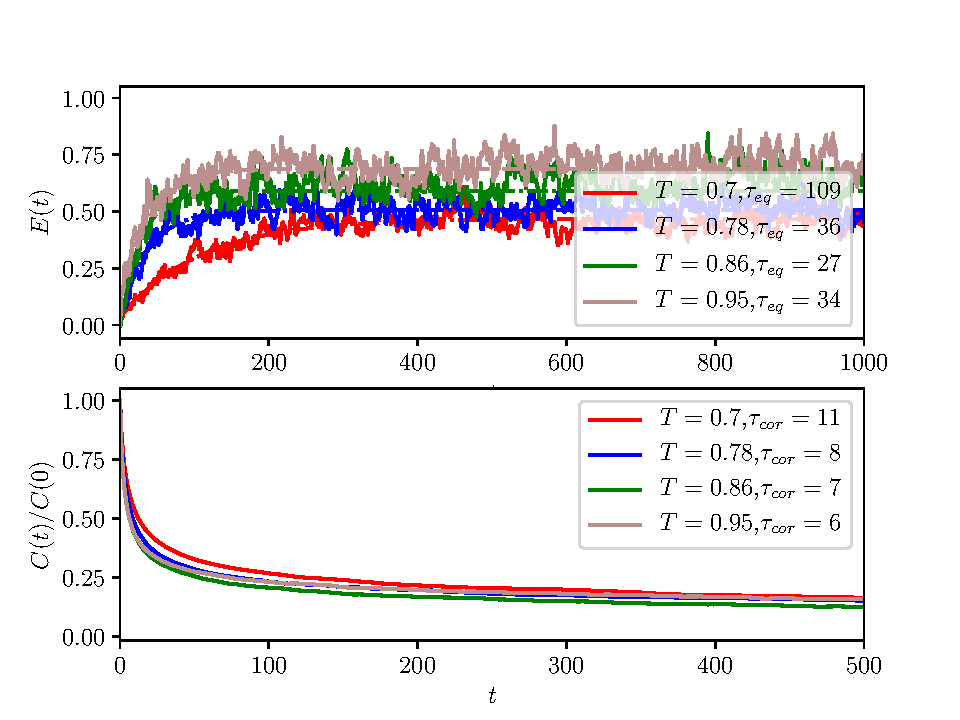
\includegraphics[scale=1]{numerical/sos-kaw-eq-cor.pdf}
	\caption{Courbe de l'énergie (haut) et fonction d'auto-corrélation (bas) dans avec un \textbf{paramètre d'ordre conservé} à partir de la condition initiale. Le temps d'équilibrage (en étapes de Monte Carlo) diminue avec la température, tandis que le temps de corrélation reste relativement constant. Le temps de corrélation est similaire à la dynamique de Glauber, bien que l'équilibrage soit plus long à se faire.}
	\label{eq-kaw}
\end{figure}
	
La diffusion des particules - par exemple un polymère dans un solvant - est une dynamique locale qui conserve le paramètre d'ordre du notre système, nommément la magnétisation $m$. Dans ce cas, on choisit au hasard de manière uniforme deux colonnes $h_i$ et $h_{i+1}$ dans lesquelles on va essayer d'échanger une particule entre les deux colonnes. Afin de respecter le bilan détaillé, il faut que la probabilité de choisir le mouvement $h_i \rightarrow h_{i+1}$ soit égale à $h_{i+1} \rightarrow h_i$. On peut juste définir à nouveau "l'ajout" d'une colonne vers ou à partir de l'autre via la transformation $h_i \rightarrow h_i + \alpha$ et $h_{i+1} \rightarrow h_{i+1} - \alpha$ (avec $\alpha=\pm 1$), en respectant toujours les conditions aux bords en $y$. Trois termes dans l'énergie sont modifiées\footnote{Comme précédement, il existe une version booléenne de l'équation, mais sa longueur n'offre aucun avantage en terme d'implémentation dans le code comparé au gain de temps de CPU engendré.}
\begin{align}
	\Delta E = &|h_{i-1}-(h_i \pm 1)| + |h_{i+1} \pm 1 -(h_i \pm 1)| + |h_{i+1}\pm 1-(h_{i+2} )| \\
	- &|h_{i-1}-h_i| - |h_{i+1}-h_i| - |h_{i+1}-h_{i+2}|
\end{align}

La magnétisation totale est ainsi conservée, tandis que la largeur de l'interface $\sigma$ se calcule par
\begin{align}
	\Delta \sigma = 2 \alpha  + 1
\end{align}

	\subsection{Dynamique hors-équilibre}
L'ensemble grand-canonique ne nous permet d'avoir un système qu'à l'équilibre, puisqu'il est traduit par une dynamique non-locale. Seule une dynamique locale comme la dynamique de Kawasaki peut nous donner des états hors-équilibre. L'implémentation la plus simple est d'introduire un terme de cisaillement dans notre modèle lorsque l'on décide de bouger une particule. Ce cisaillement diminue l'énergie du micro-état lorsque la particule bouge dans un sens et l'augmente si elle bouge dans l'autre sens, ce qui brise le bilan détaillé. De nombreux travaux sur les systèmes hors-équilibre dans le modèle d'Ising ont été produits \cite{smith_interfaces_2008} présentant la diminution de la largeur de l'interface lorsque le cisaillement est produit de manière parallèle. 
On peut définir deux espèces de cisaillement parallèles.
Le premier genre de cisaillement se produit aux bords d'un liquide non-visqueux, ce qui ne permet de bouger que les particules aux bords du système : il n'est donc pas adaptable à un système infini ou semi-infini. Pour un système de taille $L$ et pour un module de cisaillement de $f$, la différence d'énergie supplémentaire est 
\begin{align}
	\Delta E_{bord} = f [ (h_i == 1 || h_{i+1} == L-1) - (h_i == L-1 || h_{i+1} == 0)  ]
\end{align}
Le second genre de cisaillement se produit aux bords d'un fluide permettant un transport visqueux, ce qui entraîne un cisaillement proportionnel à la distance aux bords comme sur la figure \ref{snap-ising-shear}. En supposant que le cisaillement est nul au niveau de l'interface et que les particules vont à gauche dans la partie basse du système (et à droite dans la partice haute du système), on obtient alors
\begin{align}
	\Delta E_{prop} = f h_i
\end{align}
Cependant, pour des raisons de facilité de calcul plus tard afin de comparer les simulations numériques aux résultats analytiques, on utilise un cisaillement uniforme qui pousse les particules dans un sens. Ce type de système correspond à un flux laminaire, par exemple dû à la gravité face à une interface verticale qui tire les particules vers le bas. La différence d'énergie devient
\begin{align}
	\Delta E_{uni} = \alpha f
\end{align}
où $\alpha = 1$ si la particule va vers la droite, $-1$ sinon. 
		
	\subsection{Modèle POP}		

Dans le modèle POP, le modèle n'est plus structuré en fonction des sites $i$ mais bien des particules $\sigma_(n) = i$, la hauteur d'un site\footnote{Cette hauteur est mise à jour à chaque étape mouvement d'une particule dans un second tableau.} devenant alors
\begin{align}
	h_i = \sum_{n=0}^N \delta_{\sigma_n,i}
\end{align}

Lors d'une dynamique de Kawasaki, à chaque étape, on choisit au hasard une particule parmi les $N$ présentes dans le système pour la déplacer d'une colonne. 

Il est également possible de donner des constantes de diffusion différentes à chaque particule\footnote{Grâce à la construction d'un générateur via \textit{random::discrete\_distribution} où chaque particule a une probabilité différente d'être sélectionnée. }  afin d'émuler différents types de particules. 

La question est plus délicate lorsqu'il s'agit d'une dynamique de Glauber. Puisque chaque particule a une probabilité d'être sélectionnée pour être détruite, comment choisir la probabilité d'ajouter une particule au système ? À l'équilibre, le flux de particules entrantes est égale au flux de particules sortantes, c'est-à-dire $p_{ajout}= p_{retrait} = 0.5\%$. Dans ce cas, il suffit de choisir un booléen au hasard, puis détruire une particule et son label ou ajouter une particule à un site particulier. L'avantage de la dynamique conservée est qu'il n'est pas nécessaire de reconstruire une distrubtion pRNG à chaque étape, même si le constructeur est rapide \footnote{Le constructeur a une complexité en $\mathcal{O}(n)$ au pire. \url{http://www.cplusplus.com/reference/random/discrete_distribution/discrete_distribution/}}.

%%%%%%%%%%%%%%%%%%%%%%%%%%%%%%%%%%
\section{Conclusion}
%%%%%%%%%%%%%%%%%%%%%%%%%%%%%%%%%%

Dans ce chapitre nous avons décrit les différentes méthodes de calcul numérique qui vont de pair avec le modèle A et le modèle B, et la manière de mesurer les observables ainsi que leur barre d'erreur. Dans la pratique, les temps de corrélation sont si faibles qu'il suffit de faire environ $10^7$ étapes de Monte Carlo afin d'obtenir de bonnes statistiques, ce qui en une dimension, est extrêmement rapide. La rapidité des simulations dans le modèle SOS nous permet ainsi d'étudier une très vaste plage de paramètres, que ce soit pour différentes températures, cisaillements, hauteurs maximales ou champs externes. 
mux
